\chapter*{Rückblick und Ausblick}
\addcontentsline{toc}{chapter}{Rückblick und Ausblick}

Der vorgegebene Rahmen der Maturaarbeit in Bezug auf Umfang,
Nachvollziehbarkeit und Erstellungsdauer schränkte die verschiedenen Ideen zu dieser
Arbeit markant ein. Ursprünglich war angedacht, eine deutlich umfangreichere
Problemstellung zu bearbeiten. Aus diesem Grund wurde das eigentliche Potenzial von
TensorFlow und Keras bei Weitem nicht ausgeschöpft. Dadurch könnte ein falscher
Eindruck vom eigentlichen Potenzial dieser Tools entstehen. Wichtig ist daher zu
erkennen, dass TensorFlow und Keras zu weit mehr im Stande sind, als das
dargelegte Anwendungsbeispiel vermuten lässt.
\para{}
Daher soll an dieser Stelle exemplarisch aufgezeigt werden, welche
weiteren Anwendungen in einem grösseren Rahmen und unter Verwendung von
TensorFlow und Keras ebenfalls hätten bearbeitet werden können.

\section*{Variational Autoencoder}
\begin{wrapfigure}{L}{2cm}
  \qrcode[height=2cm]{https://www.youtube.com/watch?v=9zKuYvjFFS8}
\end{wrapfigure}
Wie im Vorwort erwähnt, bestand der ursprüngliche Plan dieser Arbeit
darin, einen \keyword{Variational Autoencoder} (VAE) zu implementieren. Dieser sollte genutzt werden,
um künstlich generierte Bilder von menschlichen Gesichtern zu erzeugen.
Dies ist möglich, da es sich bei einem VAE um ein sogenanntes
\keyword{Generatives Modell} handelt.
\para{}
Generative Modelle sind in der Lage, anhand
von einem existierenden Datensatz neue Dateneinträge zu generieren. Diese neuen Daten
weisen einen ähnlichen Charakter auf wie der ursprüngliche Datensatz. Diese sind
jedoch nicht in ihm enthalten.
\para{}
Ein VAE erweitert das Grundkonzept eines normalen Autoencoders. Beim VAE ist das
Encoding (Repräsentation) eine stochastische Verteilung, welche den entwickelten
Code darstellt.
Auf diese Weise wird bezweckt, dass Codes, welche im Repräsentationsraum nahe beieinander liegen, auch ähnliche
Decodings (Rekonstruktionen) erzeugen. Dadurch wird der Repräsentationsraum
kontinuierlich (siehe Abb. \refbox{fig:vae}). So können neue zufällige Codes
rekonstruiert werden, welche sinnvolle Decodings erzeugen. Auf diese Weise agiert der Decoder als generatives
Modell. Wenn beispielsweise ein VAE mit menschlichen Gesichtern
trainiert würde, könnten neue zufällige Codes rekonstruiert werden, welche dann
neue, noch nie gesehene Gesichter produzieren würde.
\para{}
Eine verständliche und gute Erklärung bietet der Youtube-Kanal
``Arxiv-Insights'' in seinem Video ``Variational Autoencoder'' (siehe QR-Code).

\begin{figure}[h!]
  \centering
  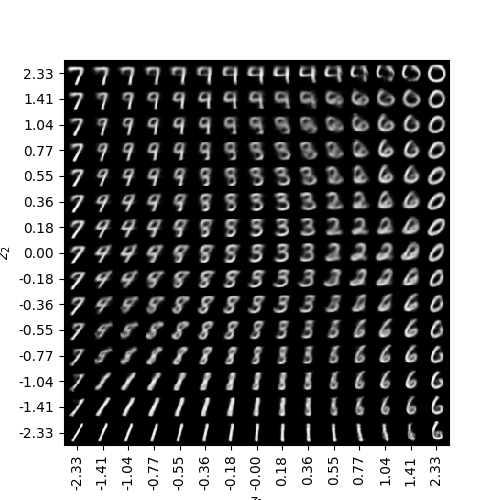
\includegraphics[width=0.4\textwidth]{vae.png}
  \caption{Decodingraum eines VAE trainiert auf MNIST: Ähnliche Ziffern sind
    nahe beieinander \cite{res:vae}}
  \label{fig:vae}
\end{figure}

\cite{wiki:autoencoder}

\section*{Generative Adversial Networks}
Ein weiteres Generatives Modell sind sogenannte \keyword{Generative Adversial
  Networks} (GANs). Sie sind der anerkannte Status Quo, was generative KNNs
anbelangt.
\para{}
Das Grundkonzept ihrer Funktionsweise lautet wie folgt: Ein GAN besteht aus zwei
KNNs, welche miteinander konkurrieren. Das eine Modell, der
\keyword{Diskriminator}, kämpft gegen das andere Modell, den \keyword{Generator}.
Die Aufgabe des Generator ist es, Daten zu generieren, welche möglichst stark
dem Trainingsdatensatz ähneln. Der Diskriminator bekommt entweder
ein Sample aus dem Trainingsdatensatz vorgelegt oder ein generiertes.
Er muss dann entscheiden, ob es echt oder generiert ist. Beide Netzwerke lernen so,
immer besser in ihrer Tätigkeit zu werden und betreiben gewissermassen einen Wettbewerb.
\para{}
NVIDIA hat 2019 ein Paper veröffentlicht, in welchem sie ein GAN implementiert
haben. Dieses Modell generierte Bilder von menschlichen Gesichtern. Die
Ergebnisse sind von Auge nicht von echten Fotos zu unterscheiden.
In Abbildung \refbox{fig:nvidia_gan} ist ein Auszug an generierten Bildern dargestellt.

\begin{figure}[h!]
  \centering
  \includegraphics[height=0.5\textwidth]{gan.png}
  \caption{generierte Gesichter von NVIDIAs GAN \cite{paper:gan}}
  \label{fig:nvidia_gan}
\end{figure}
\para{}
Quellen: \cite{paper:gan}

\section*{Frameworks}
\subsection*{TensorFlow 2.0}
TensorFlow befindet sich momentan in einer grossen Überarbeitungsphase. Es
wächst gewissermassen aus seinen Kinderschuhen heraus. Es handelt sich dabei um das
TensorFlow 2.0 Update. Bereits zum Zeitpunkt des Verfassens dieser Arbeit
existiert eine Entwicklungsversion von TF 2.0, jedoch läuft diese noch nicht
völlig stabil. Sobald TF 2.0 offiziell freigegeben wird, ist zu empfehlen,
davon Gebrauch zu machen. In dieser Überarbeitung werden viele Relikte aus den
ursprünglichen TensorFlow Versionen entfernt, welche für Verwirrung sorgen
könnten. Somit entsteht ein in sich stimmiges Framework, welches einen höheren
Komfort aufweisen soll.
\para{}
Quelle: \cite{net:tf_2.0}

\subsection*{Alternativen}
Es gibt neben TensorFlow und Keras noch weitere Frameworks, welche sich für
Maschinelles Lernen eignen. Die meisten davon sind ebenfalls hauptsächlich auf Deep
Learning ausgelegt. Sie machen auch Gebrauch von der cuDNN-Bibliothek
von NVIDIA (erwähnt in Anhang \refbox{sec:anhang_tf}). Somit weisen sie
ähnlich performante Implementierungen wie TF auf. Vorteile können in der
Intuition und Einfachheit der Bedienung liegen. Viele Privatpersonen bevorzugen
aus diesem Grund \keyword{PyTorch} gegenüber TF.
Weitere erwähnenswerte Frameworks sind: Caffe, Scikit-Learn, Sonnet.
\para{}
Quelle: \cite{book:hands-on}


\chapter*{Schlusswort}
\addcontentsline{toc}{chapter}{Schlusswort}

Rückblickend war es für mich weitestgehend ein Vergnügen, eine Maturaarbeit zum
Thema Maschinelles Lernen schreiben zu dürfen. Die Theorieabschnitte zu
verfassen, bereitete mir wirklich viel Spass. Am Ende ein funktionierendes
Programm erstellt zu haben, war ebenfalls ein Erfolgserlebnis für mich.
Inhaltlich war es aber auch eine Herausforderung, die mich bis
zum Schluss sehr umfassend beschäftigt hat, obwohl ich schon zu Beginn viele
Stunden in diese Arbeit investiert habe. Durch mein privates Interesse am
Programmieren und meine Praktika an der Universität Basel sowie bei Adobe konnte
ich mit guten Grundlagen in das Thema einsteigen. Allerdings musste ich rasch
feststellen, dass es sich um ein geradezu unerschöpfliches Thema handelt. Vor
allem die mathematische Fundierung gestaltete sich aufwändiger als ich erwartet
habe.
\para{}
Reizvoll war ebenfalls, sich detailliert mit der aktuellen Fachliteratur
auseinanderzusetzen und erste Eindrücke vom wissenschaftlichen Arbeiten zu
erhalten. Angesichts der Breite des Themas war die thematische Einschränkung ein
sinnvoller Schritt. Ich merkte rasch, dass mein ursprünglicher Anspruch, Bilder
von menschlichen Gesichtern zu generieren, aufgrund des mathematischen Umfangs
den Rahmen einer Maturaarbeit gesprengt hätte.
\para{}
Die Faszination für das Thema und die zahlreichen
Anwendungsmöglichkeiten geben mir die Gewissheit, dass ich auch inskünftig
diesem Fachgebiet verbunden bleiben möchte. So bildet meine Maturaarbeit einen
ersten Mosaikstein, auf den ich gerne zurückschauen werde.

% ---------------------------------

\begin{appendices}

\chapter{Gradientenverfahren}\label{sec:anhang_gd}
Das Gradientenverfahren ist ein numerisches Verfahren, um Funktionen $f(x_1,
x_2, \ldots, x_n)$ vom Typ $\set{R}^n \to \set{R}$ (wie z. B. die Fehlerfunktion)
zu minimieren.
Dies geschieht, indem ein Startpunkt (Ortsvektor) $\vec{p}_0$ gewählt wird, dessen
Komponenten den Input von $f(\vec{p}_0)$ darstellen.
Nun werden iterativ neue Punkte $\vec{p}_t$ gesucht, welche immer näher beim lokalen Minimum liegen, also Punkte, die den Funktionswert $f(\vec{p}_t)$ immer kleiner werden lassen.
Dies wird durchgeführt, bis der Punkt genügend nahe beim lokalen Minimum ist.
\para{}
Dafür muss ein Vektor $\vec{b}_t$ bestimmt werden, welcher auf den Punkt $\vec{p}_t$ addiert einen neuen Punkt $\vec{p}_{t+1}$ bildet,
bei dem der Funktionswert $f(\vec{p}_{t+1})$ kleiner ist als der von $f(\vec{p}_t)$.
Dies geschieht am effizientesten, wenn $\vec{b}_t$ in die Richtung der stärksten Funktionswertabnahme zeigt.

Hierzu wird der sogenannten \keyword{Gradient} $\vecf{\nabla}$ verwendet,
für den wiederum partielle Ableitungen benötigt werden.
\para{}
\begin{defbox}{Partielle Ableitungen}\label{ref:partielle_ableitungen}
  Partielle Ableitungen sind eine Erweiterung der ``normalen'' Ableitungen auf
  multidimensionale Funktionen $f(\vec{x}) = f(x_1,\ldots,x_n): \set{R}^n \to \set{R}$.
  Man leitet dabei nur nach einem Argument $x_i$ ab und betrachtet die restlichen Argumente als Konstanten.
  Es gelten die gleichen Ableitungsregeln wie bei der nicht-partiellen Ableitung.
  Die partielle Ableitung einer Funktion $f(x_1,\ldots,x_n)$ bezüglich einer
  Variable $x_i$ in einem Punkt $\vec{a} = \trans{\begin{pmatrix} a_1 & \cdots & a_n \end{pmatrix}}$
  ist analog zur normalen Ableitung folgendermassen definiert:
  \begin{equation*}
    \partderiv{f}{x_i}(\vec{a}) \coloneqq \lim_{h \to 0} \frac{f(a_1,\ldots,a_i + h,\ldots,a_n)-f(a_1,\ldots,a_i,\ldots,a_n)}{h}
  \end{equation*}
  Geometrisch ist dies die Steigung der Tangente an die Kurve der Funktion $f$ im Punkt
  $\vec{a}$. Die Tangente liegt in der Richtung der Achse des Parameters $x_i$,
  nach welchem abgeleitet wurde.
\end{defbox}
\\
\begin{defbox}{Gradient}
  Der Gradient $\vecf{\nabla}$ ist ein Differentialoperator, der auf eine
  skalare Funktion $f(\vec{x}) = f(x_1,\ldots,x_n): \set{R}^n \to \set{R}$
  angewendet, das Skalarfeld auf das Gradientenfeld (Vektorfeld) abbildet.
  Um das Gradientenfeld $\vecf{\nabla}f$ der Funktion $f$ zu bilden, fasst man alle
  partiellen Ableitungen der Funktion $f$, nach jedem Argument $x_i$, in einem
  Vektor zusammen.
  Um nun einen partikulären Vektor zu bestimmen, berechnet man den Gradienten in einem spezifischen Punkt
  $\vec{p} = \trans{\begin{pmatrix} p_1 & \cdots & p_n \end{pmatrix}}$:
  \begin{equation*}
    \vecf{\nabla}_{\vec{x}} f(\vec{p}) =
    \begin{pmatrix}
      \ds\partderiv{f}{x_1}(\vec{p}) \\
      \vdots \\
      \ds\partderiv{f}{x_n}(\vec{p}) \\
    \end{pmatrix}
  \end{equation*}

  Geometrisch ist der Gradient $\vecf{\nabla}f(\vec{p})$ einer Funktion $f$ in
  einem Punkt $\vec{p}$ der Vektor, welcher in die Richtung des steilsten
  Anstiegs von $f$ zeigt. Sein Betrag gibt die Stärke des Anstiegs an.
\end{defbox}
\\
\begin{examplebox}{Beispiel für partielle Ableitungen}
  Als Beispiel wird die Funktion $f(x,y) = x^2 + y^2 - 2$ betrachtet, welche von
  den Variablen $x$ und $y$ anhängt.
  Um die partielle Ableitung bezüglich $x$ zu bestimmen, muss $y$ als konstant
  betrachtet werden. Beispielsweise kann man $y=0$ wählen, damit die Funktion
  $g(x) = f(x,0) = x^2 - 2$ nur noch von der Variable $x$ abhängt.
  Leitet man nun nach $x$ ab, erhält man:
  $\deriv{g(x)}{x} = g'(x) = 2x$.\\
  Dies entspricht der partiellen Ableitung von $f$ nach $x$:
  \[ \partderiv{f(x,y)}{x} = 2x \]
  Die partielle Ableitung von $f$ nach $y$ lautet entsprechend:
  \[ \partderiv{f(x,y)}{y} = 2y \]
\end{examplebox}
\\
\begin{examplebox}{Gradientenbeispiel}
  Als Beispiel für den Gradienten wird die Funktion $f(x,y) = x \cdot \exp(-x^2 - y^2)$ betrachtet.
  Werden die partiellen Ableitungen nach den Argumenten $x$ und $y$ gebildet,
  so erhält man (Kettenregel und Produktregel):
  \[ \partderiv{f}{x} = \exp(-x^2 - y^2) \cdot (1-2x^2) \]
  \[ \partderiv{f}{y} = \exp(-x^2 - y^2) \cdot (-2xy) \]
  Diese beiden partiellen Ableitungen werden zum Gradient $\vecf{\nabla} f$ zusammengefasst:
  \[ \vecf{\nabla}f(x,y) =
    \begin{pmatrix}
      \ds\partderiv{f}{x} \\[8pt]
      \ds\partderiv{f}{y} \\
    \end{pmatrix}
    =
    \begin{pmatrix}
      \exp(-x^2 - y^2) \cdot (1-2x^2) \\[5pt]
      \exp(-x^2 - y^2) \cdot (-2xy) \\
    \end{pmatrix}
 \]
 In der unterstehenden Abbildung ist das Konturdiagramm der Funktion $f$
 zusammen mit dem Gradientenfeld (blaue Vektoren) dargestellt.

  \begin{center}
    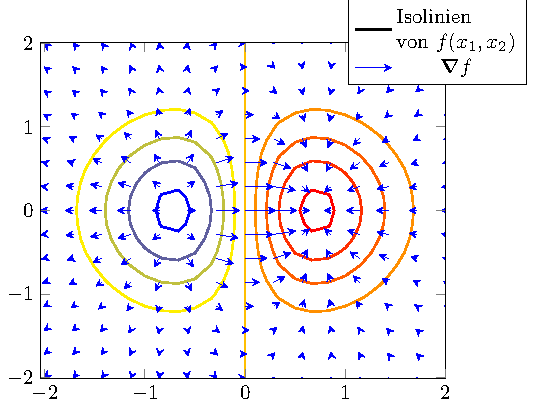
\includegraphics[width=0.68\textwidth]{grad.pdf}
    % \caption{ein Skalarfeld als Konturdiagramm mit zugehörigem Gradientenfeld}
  \end{center}
\end{examplebox}
\para{}
Da der Gradient also in die Richtung des steilsten Anstiegs zeigt, sollte der Vektor
$\vec{b}_t$ gerade in die entgegengesetzte Richtung zeigen. Demnach sollte er in die Richtung des negierten Gradienten der Funktion $f$ im Punkt $\vec{p}_t$ weisen.
Jetzt kann das iterative Annähern an das lokale Minimum folgendermassen beschrieben
werden:
\\
\begin{equation}\label{eq:gradientdescent}
  \vec{p}_{t+1} = \vec{p}_t - \alpha \cdot \vecf{\nabla} \mathit{f}(\vec{p}_t)
\end{equation}
\\
Dabei stellt $\alpha$ einen Proportionalitätsfaktor dar, welcher die
Schrittgrösse beim Abstieg bestimmt.

\ifcp%
\begin{figure}[h!]
  \centering
  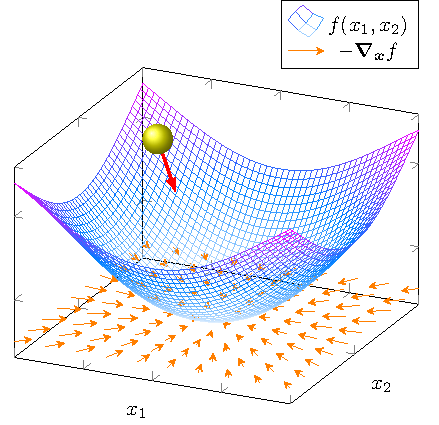
\includegraphics[width=0.5\textwidth]{gd.pdf}
  \caption{Visualisierung des Gradientenabstiegs: Ein Ball rollt das
    Gradientenfeld hinab in das lokale Minimum.}
\end{figure}
\fi%

Während des Gradientenverfahrens konvergiert der Punkt $\vec{p}_t$ zu einem
beliebigen \textit{lokalen} Minimum, abhängig davon, wie der Startpunkt
$\vec{p}_0$ gewählt wurde.
\para{}
Quellen: \cite{book:hands-on} \cite{Nielsen}

\chapter{Herleitung der Rückwärtspropagierung für KNNs}\label{sec:anhang_bp}
Da ein KNN, wie der Name schon andeutet, vernetzt ist, können die partiellen
Ableitungen einer Schicht anhand seiner Nachbarsschichten berechnet werden.
Dies ist auch der namensgebende Grundgedanke der Rückwärtspropagierung: Man
beginnt damit, die partiellen Ableitung der letzten Schicht zu bestimmen und
berechnet dann retrograd Schicht für Schicht die vorherigen
partiellen Ableitungen bis zur Inputschicht. \\
Dies geschieht unter Anwendung der Kettenregel der Ableitungen.
Es ist sinnvoll, für das Aufstellen dieser Gleichungen das Netzwerk als
\keyword{Computational Graph} zu betrachten.
\para{}
\begin{infobox}{Computational Graph}
  Ein Computational Graph ist die Darstellung einer Verkettung von Funktionen als Netzwerk von Operationen.
  Die Knoten im Graph stellen Variablen dar und die Pfade, welche die Knoten
  verbinden, sind die Funktionen, welche die Variablen aufeinander abbilden. Die
  Funktion wird auf die Variable angewendet, von der der Pfad ausgeht. Der Knoten,
  in welchem der Pfad endet, nimmt dann den Funktionswert an. Falls
  mehrere Pfade in einem einzigen Knoten enden, werden die einzelnen Werte der Pfade
  zusammenaddiert, um die Variable zu bilden. In diesem Graphen sind die
  Abhängigkeiten der Variablen voneinander gut ersichtlich. Auf dieser Basis können mithilfe
  der Kettenregel die Ableitungen unkompliziert bestimmt werden.
\end{infobox}
\para{}
\begin{examplebox}{Beispiel eines Computational Graph}
  Untenstehend ist ein Beispiel eines Computational
  Graph zusammen mit der Herleitung der partiellen Ableitungen dargestellt.
  \para{}
  \begin{center}
    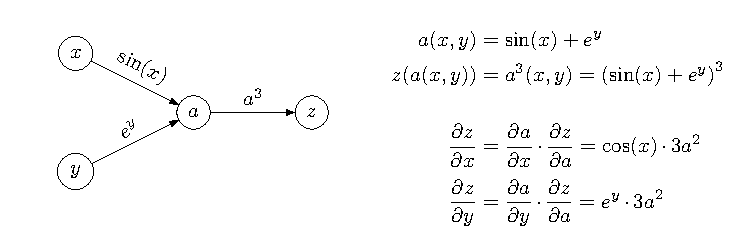
\includegraphics[width=0.8\textwidth]{compgraph.pdf}
    % \caption{Computational Graph einer exemplarischen Verkettung von Funktionen}
  \end{center}
\end{examplebox}
\para{}
\pagebreak
Der erste Schritt der Rückwärtspropagierung besteht darin, dass die partiellen Ableitungen $\ds\partderiv{C}{z_j^l}$
der Kostenfunktion $C$ bezüglich den gewichteten Summen $z_j^l$ aller Schichten
berechnet werden müssen. Daraus lassen sich dann später die partiellen Ableitungen
bezüglich den Gewichten $\ds\partderiv{C}{w_{j,k}^l}$ und bezüglich den Neigungen
$\ds\partderiv{C}{b_j^l}$ ermitteln.
\para{}
Zur Übersichtlichkeit definiert man einen \keyword{Fehler} $\delta_j^l$ für
jedes $j$-te Neuron in jeder $l$-ten Schicht, welcher die partielle Ableitung bezüglich der
gewichteten Summe dieses Neurons darstellt (siehe Gl. \refbox{eq:RP0}). Ebenfalls definiert man analog einen Fehlervektor
$\vec{\delta}^l$, welcher alle Fehler $\delta_j^l$ einer Schicht $l$
zusammenfasst (siehe Gl. \refbox{eq:RP0a}). Nun heisst es, diesen Wert für jedes Neuron jeder Schicht zu
berechnen.
\\
\begin{gather}
  \tag{RP0}\label{eq:RP0} \delta_j^l \coloneqq \partderiv{C}{z_j^l} \\
  \tag{RP0a}\label{eq:RP0a} \vec{\delta}^l \coloneqq \trans{\begin{pmatrix} \ds\partderiv{C}{z_1^l} & \ds\partderiv{C}{z_2^l} & \cdots & \ds\partderiv{C}{z_{|l|}^l} \end{pmatrix}}
\end{gather}
\\
Da die Kostenfunktion unmittelbar auf die letzte Schicht $L$ angewendet wird, beginnt
dort auch die Berechnung des Fehlers $\vec{\delta}^L$.
Nun wird ein Computational Graph aufgestellt, um die partiellen Ableitungen zu bestimmen.
\para{}
\begin{figure}[h!]
  \centering
  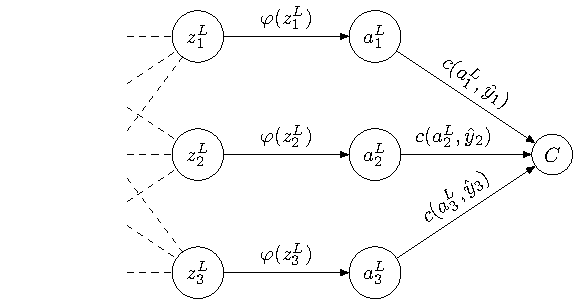
\includegraphics[width=0.7\textwidth]{del_l.pdf}
  \caption{Computational Graph zur Berechnung von $\vec{\delta}^L$}
  \label{fig:cg_L}
\end{figure}
\para{}
Aus dem Computational Graph der Abbildung \refbox{fig:cg_L} kann entnommen werden, dass die Kosten $C$ eine Funktion
in Abhängigkeit von den letzten Aktivierungen $a_j^L$ ist. Diese ist wiederum
eine Funktion in Abhängigkeit von der jeweiligen gewichteten Summe $z_j^L$.
Somit kann mithilfe der Kettenregel die Beziehung \refbox{eq:RPh1}
aufstellt werden.
\\
\begin{equation}\label{eq:RPh1}
  \delta_j^L = \partderiv{C}{z_j^L} = \partderiv{C}{a_j^L} \cdot \partderiv{a_j^L}{z_j^L}
\end{equation}
\\
Da $a_j^L$ durch die Anwendung der Aktivierungsfunktion $\varphi$ auf $z_j^L$
gebildet wird, ist $\ds\partderiv{a_j^L}{z_j^L}$ die Ableitung der Aktivierungsfunktion
$\varphi'(z_j^L)$. Auf diese Weise lässt sich die erste \refbox{eq:RP1} von vier
wichtigen Gleichungen für die Rückwärtspropagierung herleiten.
\\
\begin{equation}\tag{RP1}\label{eq:RP1}
  \delta_j^L = \partderiv{C}{a_j^L} \cdot \varphi'(z_j^L)
\end{equation}
\\
Um diese Ausdrücke wieder in Matrixschreibweise zu realisieren,
welche die ganze Schicht $L$ zusammenfasst, muss eine
neue Operation eingeführt werden: das Hadamard-Produkt.

\begin{defbox}{Hadamard-Produkt}
  Das Hadamard-Produkt (auch elementweises Produkt) ist eine spezielle Multiplikation zweier gleichgrosser Matrizen
  $\mat{A} \in \set{R}^{m \times n}$ und $\mat{B} \in \set{R}^{m \times n}$.
  Die resultierende Matrix ergibt sich aus der elementweisen Multiplikation der Ausgangsmatrizen.

  \begin{minipage}{0.5\textwidth}
    \begin{equation*}
      \mat{A} \odot \mat{B} =
      \begin{pmatrix}
        \matelem{A}_{1,1} \matelem{B}_{1,1} & \cdots & \matelem{A}_{1,n} \matelem{B}_{1,n} \\[0.3em]
        \vdots & \ddots & \vdots \\[0.3em]
        \matelem{A}_{m,1} \matelem{B}_{m,1} & \cdots & \matelem{A}_{m,n} \matelem{B}_{m,n} \\[0.3em]
      \end{pmatrix}
      \in \set{R}^{m \times n}
    \end{equation*}
  \end{minipage}
  %
  \begin{minipage}{0.5\textwidth}
    \begin{equation*}
      \vec{v} \odot \vec{w} =
      \begin{pmatrix}
        v_1 w_1 \\
        \vdots \\
        v_n w_n
      \end{pmatrix}
    \end{equation*}

  \end{minipage}
\end{defbox}
\para{}

Mit $\vecf{\varphi}'$ als die vektorisierte Ableitung der Aktivierungsfunktion
kann der Fehlervektor der letzten Schicht nach Gleichung \refbox{eq:RPh0}
berechnet werden.

\begin{equation}\label{eq:RPh0}
  \vec{\delta}^L = \trans{\begin{pmatrix} \ds\partderiv{C}{a_1^L} & \ds\partderiv{C}{a_2^L} & \cdots & \ds\partderiv{C}{a_{|L|}^L}\end{pmatrix}} \odot \vecf{\varphi}'[\vec{z}^L]
\end{equation}

Dabei ist der erste Operand des Hadamard-Produkts nichts anderes als
der Gradient $\vecf{\nabla}_{\vec{a}^L} C$ der Kostenfunktion $C$ bezüglich dem Aktivierungsvektor
$\vec{a}^L$ der letzten Schicht. Dieser Gradient kann ermittelt werden, indem die
vektorisierte Ableitungsfunktion für die gewählte Kostenfunktion gebildet wird.
Würde $C_{\text{MSE}} = \frac{1}{2|L|}(\vec{\hat{y}} -
\vec{a}^L)^2$ als Kostenfunktion gewählt werden,
ergäbe sich $\vecf{\nabla}_{\vec{a}^L} C = (\vec{a}^L - \vec{\hat{y}}) \cdot \frac{1}{|L|}$.
\para{}
Daraus folgt die kompakte Matrix-Version \refbox{eq:RP1a} der Gleichung
\refbox{eq:RP1}, welche den Fehlervektor für die letzte Schicht berechnet.
\\
\begin{equation}\tag{RP1a}\label{eq:RP1a}
  \vec{\delta}^L = \vecf{\nabla}_{\vec{a}^L}C \odot \vecf{\varphi}'(\vec{z}^L)
\end{equation}
\\
Nun soll eine rekursive Berechnungsmethode des Fehlers $\delta_j^{l-1}$
der vorherigen Schicht anhand des Fehlers $\delta_j^l$ der jetzigen Schicht
erarbeitet werden. Zu diesem Zweck ist wiederum ein Computational Graph aufzustellen
(siehe Abb. \refbox{fig:cg_L-1}).
\para{}
\begin{figure}[h!]
  \centering
  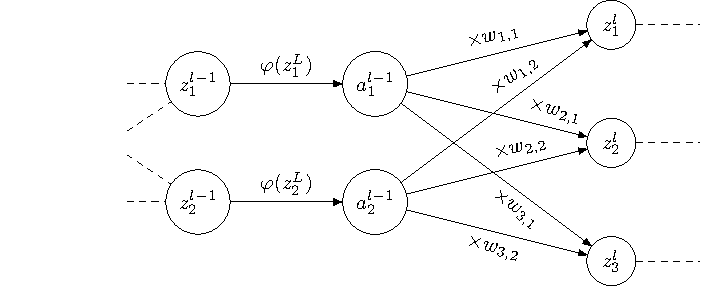
\includegraphics[width=0.7\textwidth]{del_l-1.pdf}
  \caption{Computational Graph zur Berechnung von $\delta_j^{l-1}$}
  \label{fig:cg_L-1}
\end{figure}
\para{}
Es gilt erneut die Gleichung \refbox{eq:RPh1} für die Berechnung des Fehlers $\delta_j^{l-1}$.
\\
\begin{equation}\tag{\refbox{eq:RPh1}}
  \delta_j^{l-1} = \partderiv{C}{z_j^{l-1}} = \partderiv{a_j^{l-1}}{z_j^{l-1}} \cdot \partderiv{C}{a_j^{l-1}}
\end{equation}
\\
Der erste Faktor entspricht der Ableitung $\varphi'(z_j^{l-1})$ der Aktivierungsfunktion.
Beim Übergang einer Schicht ($l-1$) zur Schicht $l$ beinflusst eine Aktivierung
$a_j^{l-1}$ alle gewichteten Summen $z_k^l$. Mit der Kettenregel folgt daher,
dass die partielle Ableitung $\ds\partderiv{C}{a_j^{l-1}}$ die Summe aller
$\ds\partderiv{C}{z_k^l} \cdot \ds\partderiv{z_k^l}{a_j^{l-1}}$ sein muss.
Daraus ergibt sich Gleichung \refbox{eq:RPh2}.
\\
\begin{equation}\label{eq:RPh2}
  \delta_j^{l-1} = \varphi'(z_j^{l-1}) \cdot \sum_{k=1}^{|l|} \left( \partderiv{C}{z_k^l} \cdot \partderiv{z_k^l}{a_j^{l-1}} \right)
\end{equation}
\\
Um die gewichtete Summe $z_k^l$ zu bilden, wird
Aktivierung $a_j^{l-1}$ der vorherigen Schicht mit den entsprechenden Gewichten
$w_{k,j}^{l-1}$ multipliziert.
Dadurch entspricht diese partielle Ableitung $\ds\partderiv{z_k^l}{a_j^{l-1}}$ gerade dem
Gewicht selbst. Desweiteren ist $\ds\partderiv{C}{z_k^l}$ per Definition der
Fehler $\delta_k^l$. Mit dieser Erkenntnis lässt sich die zweite essenzielle
Gleichung \refbox{eq:RP2} für die Rückwärtspropagierung aufstellen.
\\
\begin{equation}\tag{RP2}\label{eq:RP2}
  \delta_j^{l-1} = \varphi'(z_j^{l-1}) \cdot \sum_{k=1}^{|l|} \left( \delta_k^l \cdot w_{k,j}^{l-1} \right)
\end{equation}
\\
Auch diese Gleichung soll in der Matrixschreibweise dargestellt werden. Zu
diesem Zweck wird mit der Erweiterungen auf alle gewichteten Summen begonnen:
\\
\begin{equation*}
  \vec{\delta}^{l-1} = \vecf{\varphi}'[\vec{z}^{l-1}] \odot \trans{\begin{pmatrix} \ds\sum_{k=1}^{|l|} w_{k,1}^{l-1} \cdot \delta_k^l & \cdots & \ds\sum_{k=1}^{|l|} w_{k,|l-1|}^{l-1} \cdot \delta_k^l \end{pmatrix}}
\end{equation*}
\\
Der zweite Operand des Hadamard-Produkts ist hierbei gerade das Produkt der
Matrixmultiplikation zwischen
der transponierten Gewichtsmatrix $\trans{(\mat{W}^{l-1})}$ der Schicht ($l-1$)
und dem Fehlervektor $\vec{\delta}^l$ der Schicht $l$.

\begin{gather*}
  \trans{\begin{pmatrix} \ds\sum_{k=1}^{|l|} w_{k,1}^{l-1} \cdot \delta_k^l & \cdots & \ds\sum_{k=1}^{|l|} w_{k,|l-1|} \cdot \delta_k^l \end{pmatrix}} =
  \begin{pmatrix}
    w_{1,1}^{l-1} & w_{2,1}^{l-1} & \cdots & w_{|l|,1}^{l-1} \\
    w_{1,2}^{l-1} & w_{2,2}^{l-1} & \cdots & w_{|l|,2}^{l-1} \\
    \vdots & \vdots & \ddots & \vdots \\
    w_{1,|l-1|}^{l-1} & w_{2,|l-1|}^{l-1} & \cdots & w_{|l|,|l-1|}^{l-1}
  \end{pmatrix}
  \trans{\begin{pmatrix} \delta_1^l & \cdots & \delta_{|l|}^l \end{pmatrix}} \\[5pt]=
  \trans{\begin{pmatrix}
      w_{1,1}^{l-1} & w_{1,2}^{l-1} & \cdots & w_{1,|l-1|}^{l-1} \\
      w_{2,1}^{l-1} & w_{2,2}^{l-1} & \cdots & w_{2,|l-1|}^{l-1} \\
      \vdots & \vdots & \ddots & \vdots \\
      w_{|l|,1}^{l-1} & w_{|l|,2}^{l-1} & \cdots & w_{|l|,|l-1|}^{l-1}
    \end{pmatrix}}
  \vec{\delta}^l = \trans{(\mat{W}^{l-1})} \vec{\delta}^l
\end{gather*}
\para{}
Damit wurde die rekursive Fehlerdefinition in Matrixschreibweise
ausgedrückt. Und wir erhalten die kompakte Version \refbox{eq:RP2a} der zweiten wichtigen Formel \refbox{eq:RP2}.
\\
\begin{equation}\tag{RP2a}\label{eq:RP2a}
  \vec{\delta}^{l-1} = (\trans{(\mat{W}^{l-1})} \vec{\delta}^l) \odot \vecf{\varphi}'[\vec{z}^{l-1}]
\end{equation}
\\
In einem letzten Schritt sind nun noch die Formeln herzuleiten, mit welchen
anhand des Fehlers $\delta_j^l$ die partiellen Ableitungen der Gewichte und
der Neigungen berechnet werden können.
\para{}
Eine Neigung $b_j^l$ ist Funktionsbestandteil der entsprechenden gewichteten
Summe $z_j^{l+1}$. Somit gilt für die Neigung Formel \refbox{eq:RPh3}.
\\
\begin{equation}\label{eq:RPh3}
  \partderiv{C}{b_j^l} = \partderiv{C}{z_j^{l+1}} \cdot \partderiv{z_j^{l+1}}{b_k^l}
\end{equation}
\\
Der erste Term ist hierbei per Definition der Fehler $\delta_j^{l+1}$ und der
zweite Term lässt sich auf 1 kürzen, da die Summe $z_k^{l+1}$ nur aus
$b_k^l$ besteht und aus Summanden, welche für die partielle Ableitung als konstant gelten.
Somit entspricht die Ableitung der Neigung gerade dem Fehler, womit die
dritte \refbox{eq:RP3} von vier essenziellen Gleichungen ermittelt wurde.
\\
\begin{equation}\tag{RP3}\label{eq:RP3}
  \partderiv{C}{b_j^l} = \delta_j^{l+1}
\end{equation}
\\
Somit entspricht der Kostengradient bezüglich der Neigung dem Fehlervektor.
\\
\begin{equation}\tag{RP3a}\label{eq:RP3a}
  \vecf{\nabla}_{\vec{b^l}} C =  \vec{\delta}^{l+1}
\end{equation}
\\
Ein Gewicht $w_{j,k}^l$ ist ebenfalls ein Funktionsbestandteil der assoziierten
gewichteten Summe $z_j^{l+1}$. Dadurch gilt für die partiellen Ableitungen der
Kosten nach dem Gewicht die Gleichung \refbox{eq:RPh4}.
\\
\begin{equation}\label{eq:RPh4}
  \partderiv{C}{w_{j,k}^l} = \partderiv{C}{z_j^{l+1}} \cdot \partderiv{z_j^{l+1}}{w_{j,k}^l}
\end{equation}
\\
Dabei entspricht der erste Teil der Gleichung wieder dem Fehler $\delta_j^{l+1}$.
Die zweite partielle Ableitung ist gerade die Aktivierung $a_k^l$, da sich die
gewichtete Summe aus der Multiplikation des Gewichtes mit der Aktivierung ergibt.
Auf diese Weise entsteht die letzte der vier essenziellen Gleichungen \refbox{eq:RP4}.
\begin{equation}\tag{RP4}\label{eq:RP4}
  \partderiv{C}{w_{j,k}^l} = \delta_j^{l+1} \cdot a_k^l
\end{equation}
\\
Die Matrix-Version lässt sich als Gleichung \refbox{eq:RP4a} ausdrücken.
\begin{equation}\tag{RP4a}\label{eq:RP4a}
  \vecf{\nabla}_{\mat{W}^l} C = \vec{\delta}^{l+1} \trans{(\vec{a^l})}
\end{equation}

\begin{graybox}{Zusammenfassung Rückwärtspropagierung}
  \begin{enumerate}
    \setcounter{enumi}{-1}
  \item{Vorwärtspropagierung durchführen und dabei alle Zwischenwerte beibehalten.}
    \item{Berechnung des Fehlers $\vec{\delta}^L$ der letzten Schicht, anhand
        der Formel:
      \begin{equation}\tag{RP1a}
        \vec{\delta}^L = \vecf{\nabla}_{\vec{a}^L}C \odot \vecf{\varphi}'(\vec{z}^L)
      \end{equation}
      }
      \item{Rekursive Berechnung des Fehlers $\vec{\delta}^{l-1}$ der jeweils
          vorherigen Schicht, anhand der Formel:
          \begin{equation}\tag{RP2a}
            \vec{\delta}^{l-1} = (\trans{(\mat{W}^{l-1})} \vec{\delta}^l) \odot \vecf{\varphi}'[\vec{z}^{l-1}]
          \end{equation}
        }
      \item{Berechnung des Kostengradienten bezüglich der Neigungen, anhand der Formel:
          \begin{equation}\tag{RP3a}
            \vecf{\nabla}_{\vec{b^l}} C =  \vec{\delta}^{l+1}
          \end{equation}
        }
      \item{Berechnung des Kostengradienten bezüglich den Gewichten, anhand der Formel:
          \begin{equation}\tag{RP4a}
            \vecf{\nabla}_{\mat{W}^l} C = \vec{\delta}^{l+1} \trans{(\vec{a^l})}
          \end{equation}
        }
      \item{Gewichte und Neigung mit SGD aktualisieren}
  \end{enumerate}
\end{graybox}

\para{}
\cite{Nielsen}
\cite{rojas}
\cite{ma:deep_learning}

\chapter{Performance von TensorFlow}\label{sec:anhang_tf}
\section*{Devices}
Die Kernstücke des TensorFlow Backends sind die verschiedenen \keyword{Devices}, auf
welchen die Berechnungen ausgeführt werden. Ein Device ist jegliche Art von
Computerprozessor, auf welchem die Computational Graphs ausführt werden können.
Zu diesen Prozessoren gehören die CPU (Hauptprozessor) und die GPU
(Grafikprozessor), falls die CUDA-Version von TF installiert wurde.
\para{}
Das Backend analysiert die verfügbaren Devices und bewertete sie bezüglich
ihren Fähigkeiten. Anhand dieser Bewertung wird dann entschieden, auf
welchem Device die Berechnugen ausgeführt werden%
\footnote{
  Es ist möglich, die Graphen auf mehreren Devices gleichzeitig auszuführen und
  auf diese Weise die Modelle noch schneller zu trainieren. Dies ist jedoch erst für sehr
  aufwendige Projekte sinnvoll und erfordert ein fortgeschritteneres Verständnis.
}.
Insofern GPUs zur Verfügung stehen, wählt TF grundsätzlich immer diese, da
sie Tensoroperationen deutlich schneller als CPUs verarbeiten können.

\section*{Performance und Hardwarebeschleunigung}
Nun möchten wir die Gründe für die beachtliche Performance von TF erschliessen.
Der erste wichtige Faktor dabei ist, dass das Backend grösstenteils in C++
geschrieben ist. C++ ist eine Programmiersprache die, sehr nahe am Maschinen-Code
(engl.: low-level) ist. Somit ist der Code sehr hardwarenah und kann so
schneller ausgeführt werden. Der Nachteil besteht darin, dass die Programmiersprache
ziemlich aufwendig ist. Das bedeutet, man braucht viel Programmcode, um eine relativ einfache Idee
auszudrücken. Deshalb wurde der Client von TF in Python geschrieben, was
Abhilfe verschafft und so ein relativ einfaches Entwickeln ermöglicht.
\para{}
Der andere wichtige Aspekt für die Performance ist die sogenannte
\keyword{Hardwarebeschleunigung} (engl. hardware acceleration), von welcher TF
Gebrauch macht.
Hardwarebeschleunigung bezeichnet eine Sammlung an Methoden,
bei welchen man spezialisierte Hardware verwendet, um rechenintensive Aufgaben
schneller auszuführen. Die Architektur einer CPU ist zwar so ausgelegt, dass
sie beliebige Aufgaben ausführen kann, jedoch meistens nicht besonders
effizient. Deshalb existieren einerseits alternative externe Hardwarebausteine, wie die
GPU, welche sich für Grafikberechnungen besonders eignen.
Andererseits wurde auch die interne Architektur der CPU so angepasst, dass sie
auch spezialisierte Aufgaben besser meistert.
\para{}
Eine solche Architekturanpassung stellt die
\keyword{Parallelisierung} von Operationen dar. Dabei spaltet man eine
rechenintensive Aufgabe in viele Teilaufgaben, welche gleichzeitig in
gleicher Weise ausgeführt werden. Voraussetzung dafür ist, dass die
Teilaufgaben alle die gleichen Schritte umfassen und unabhängig voneinander bearbeitet werden können.
Ein typisches Beispiel für die Parallelisierbarkeit von Operationen ist die
Matrixmultiplikation. Möchte man eine Matrix $\mat{A} \in \set{R}^{n \times m}$ mit
einer zweiten Matrix $\mat{B} \in \set{R}^{m \times p}$ multiplizieren, muss man
praktisch $m$-mal den gleichen Schritt ausführen: Man berechnet jeweils das
Skalarprodukt zwischen der $i$-ten Zeile von $\mat{A}$ und der $i$-ten Spalte
von $\mat{B}$. Alle diese Skalarprodukte haben keinen Einfluss aufeinander und
können so unabhängig mit der gleichen Prozedur berechnet werden.
\para{}
Allgemein eignen sich Tensoroperationen zur Parallelisierung und damit zur Hardwarebeschleunigung.
Nun ist auch ersichtlich, weshalb TensorFlow als Hauptdatentyp Tensoren
verwendet.

\subsection*{CPU-Beschleunigung}
Die Hardwarebeschleunigung der CPU ist für TensorFlow nur von geringfügiger
Relevanz, da TF sich vor allem für GPU-Hardwarebeschleunigung eignet
und dafür optimiert ist. Ausserdem ist es praktisch unmöglich, die gleiche
Performance von TF mit einer CPU zu erreichen, welche mit einer GPU möglich ist.
\para{}
Die Parallelisierung auf der CPU wird einerseits durch sogenanntes \keyword{SIMD}
(``single instruction, mutiple data'') bewerkstelligt. Dies stellt ein Prinzip
dar, welches die gleiche Instruktion parallel auf mehrere Dateneinheiten
ausführt.
Andererseits werden auf der CPU die ganzen Berechnungen auf mehreren sogenannten
\keyword{Threads} ausgeführt. Da fast alle heutigen CPUs mehrere Kerne
besitzen, kann nicht nur auf einem einzigen, sondern gleich auf mehreren
Kernen gerechnet werden.

\subsection*{GPU-Beschleunigung}
Die Hardwarebeschleunigung für die Grafikkarte wird durch ein spezielles
externes Framework erreicht. TensorFlow verwendet \keyword{cuDNN} (``NVIDIA CUDA
deep learning neural network library'') eine von
NVIDIA entwickelte Programmbibliothek, um Deep Learning performant auf einer NVIDIA-GPU
auszuführen. Praktisch alle professionellen Deep-Learning-Frameworks machen
Gebrauch davon. Sie ist in der Programmiersprache
\keyword{CUDA} geschrieben, welche ebenfalls von NVIDIA entwickelt wurde. Zudem
ist sie eine zu C++ sehr ähnliche Programmiersprache, welche jedoch nicht auf
einer CPU ausgeführt wird, sondern auf einer GPU.

Quelle: \cite{net:cudnn}

% --------------------------

\chapter{GitHub}
Auf meinem GitHub-Account (LU15W1R7H) existiert ein Repository, welches verschiedene
Dateien enthält, die für die vorliegende Arbeit relevant sind.
Der mit \code{code} betitelte Ordner enthält sämtliche
Programmcodes, welche in der Arbeit erwähnt wurden. Im Ordner \code{latex}
befinden sich alle \LaTeX{}-Dateien, die zur Kompilierung der Arbeit selbst
benötigt werden. Der untenstehende QR-Code ist ein direkter Link zum
GitHub-Repository dieser Maturaarbeit.
\para{}
\begin{wrapfigure}{R}{3.5cm}
  \centering
  \qrcode[height=2cm]{https://github.com/LU15W1R7H/matura}
  \caption{QR-Code zur URL:\\ \protect\url{https://github.com/LU15W1R7H/matura}}
\end{wrapfigure}



\end{appendices}

\printbibliography[heading=bibintoc]

\addcontentsline{toc}{chapter}{Abbildungsverzeichniss}
\listoffigures

\addcontentsline{toc}{chapter}{Tabellenverzeichniss}
\listoftables

\addcontentsline{toc}{chapter}{Selbstständigkeitserklärung}
\chapter*{Selbstständigkeitserklärung}
Ich erkläre hiermit, dass ich diese Arbeit selbstständig durchgeführt und keine
anderen als die angegebene Quellen, Hilfsmittel und Hilfspersonen beigezogen
habe. Alle Textstellen in der Arbeit, die wörtlich oder sinngemäss aus Quellen
entnommen wurden, habe ich als solche gekennzeichnet.

\vspace{2cm}
\begin{center}
  \noindent\rule{5cm}{0.4pt}\\
  Luis Wirth
\end{center}


%%% Local Variables:
%%% mode: latex
%%% TeX-master: "../main"
%%% End:
